% Tento soubor nahraďte vlastním souborem s přílohami (nadpisy níže jsou pouze pro příklad)
% This file should be replaced with your file with an appendices (headings below are examples only)

% Umístění obsahu paměťového média do příloh je vhodné konzultovat s vedoucím
% Placing of table of contents of the memory media here should be consulted with a supervisor


\chapter{PIR signal recording}
\label{appendix:PIRSignal}

The training and testing data sets were done in two recording session.
The sessions included movements in several directions, shown at the
data as part of the appendix in the directory {\texttt data/}. The
type of movement can be read from the data caption.

\paragraph{First recording}
The first recording was made in a area shown at \ref{fig:measurement}.
The trajectories were concentred circles with sensor in the center
and the radius values $3m$, $6m$, $9m$ and $12m$.
The direction was either left-to-right (LR) or right-to-left (RL).
The marking of the data begins with "o", standing for older.
For example {\it 6m\_RL} is movement $6m$ from sensor right-to-left.

\begin{figure}[!ht]
\begin{center}

\includegraphics[width=0.25\textwidth]{render/measurement.png}
\caption{Measurement workplace.\label{fig:measurement}}
\end{center}
\end{figure}

Other cases are recorded as well: person walking towards ({\it C\_BF})
or walking away ({\it C\_FB}) from the sensor and no movement ({\it E}). 

\paragraph{Second recording}
After the recording, a defect was found on the device and so the data
collection was repeated. This recording has prefixes {\it c4m\_} and {\it c5m\_}
for circular movement in radiuses $4m$ and $5m$, {\it dBF\_} and {\it dFB\_}
for diagonal movement from the back to the front and from the front
to the back and {\it e\_} for no movement.

The movement is {\it LR} for movement left-to-right and {\it RL}
for right-to-left. As an example, {\it dFB\_LR\_1} is movement
for diagonal movement from the left front to the right back.

\begin{figure}[!ht]
\begin{center}
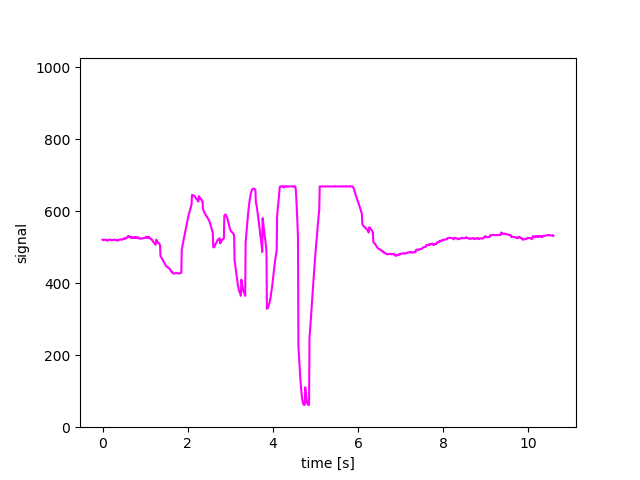
\includegraphics[width=0.3\textwidth]{../data/c4m_LR_1/c4m_LR_1_1.png}
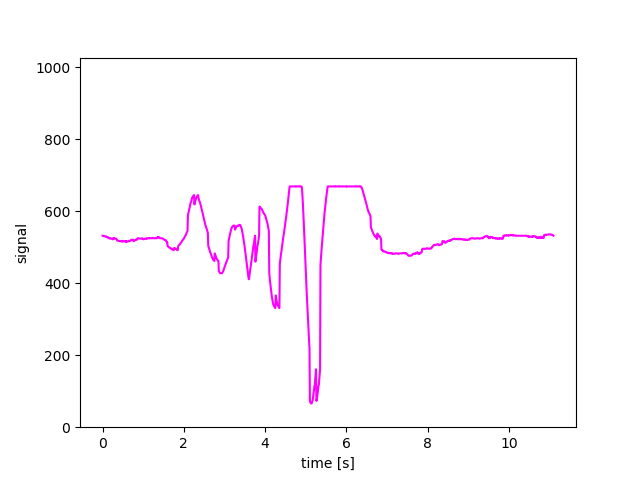
\includegraphics[width=0.3\textwidth]{../data/c4m_LR_1/c4m_LR_1_2.png}
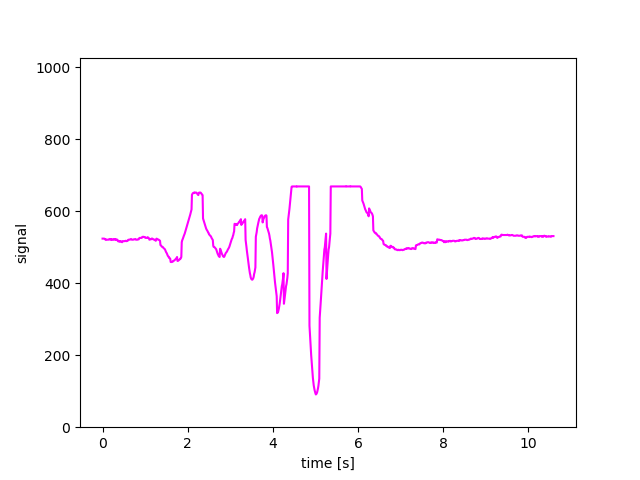
\includegraphics[width=0.3\textwidth]{../data/c4m_LR_1/c4m_LR_1_3.png}
\caption{c4m\_LR\_1.\label{fig:c4m_LR_1}}
\end{center}
\end{figure}

\begin{figure}[!ht]
\begin{center}
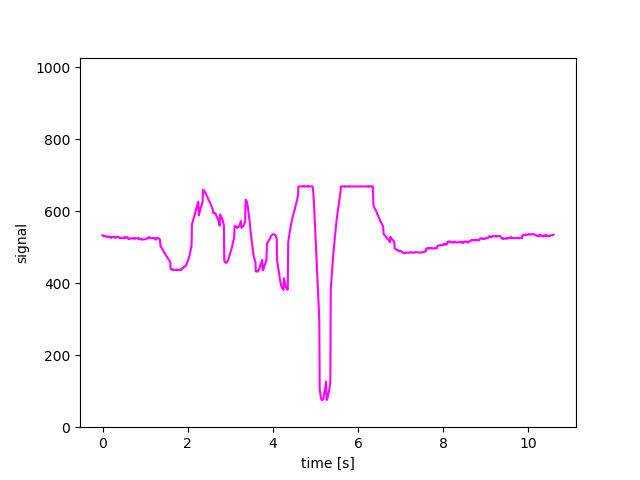
\includegraphics[width=0.3\textwidth]{../data/c4m_LR_2/c4m_LR_2_1.png}
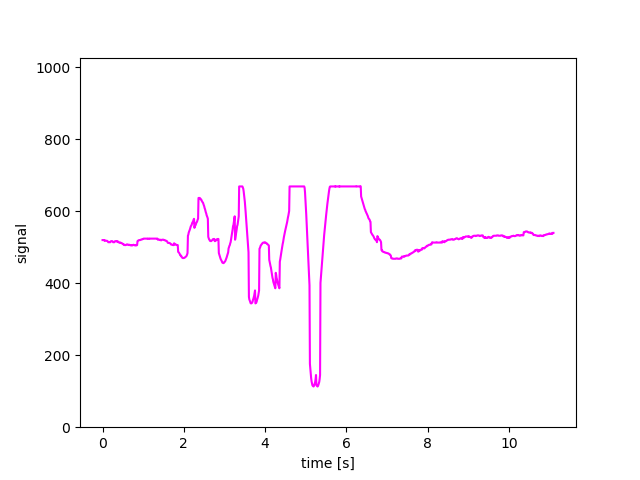
\includegraphics[width=0.3\textwidth]{../data/c4m_LR_2/c4m_LR_2_2.png}
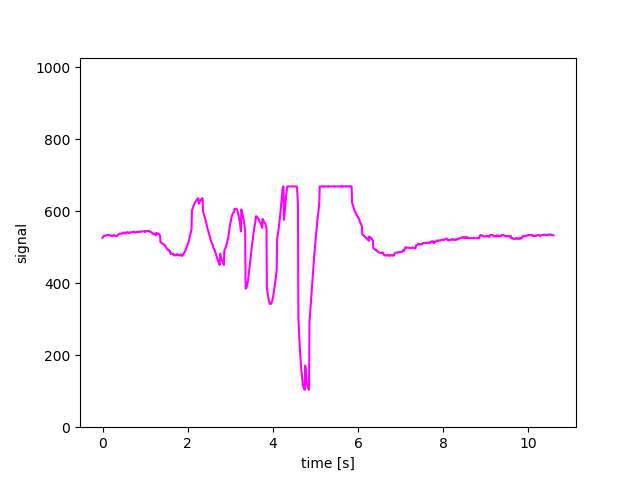
\includegraphics[width=0.3\textwidth]{../data/c4m_LR_2/c4m_LR_2_3.png}
\caption{c4m\_LR\_2.\label{fig:c4m_LR_2}}
\end{center}
\end{figure}

\begin{figure}[!ht]
\begin{center}
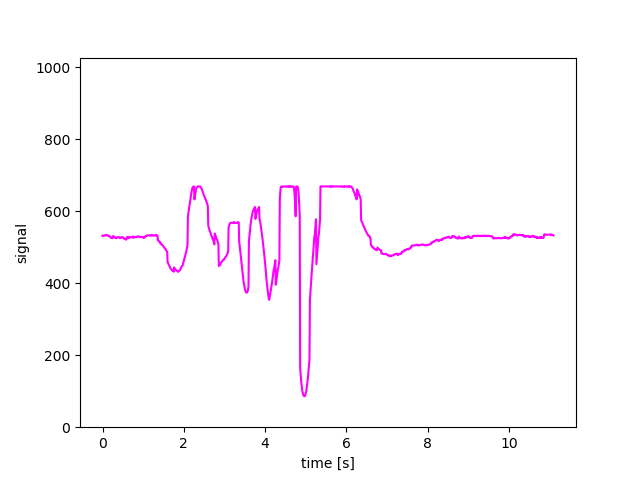
\includegraphics[width=0.3\textwidth]{../data/c4m_LR_3/c4m_LR_3_1.png}
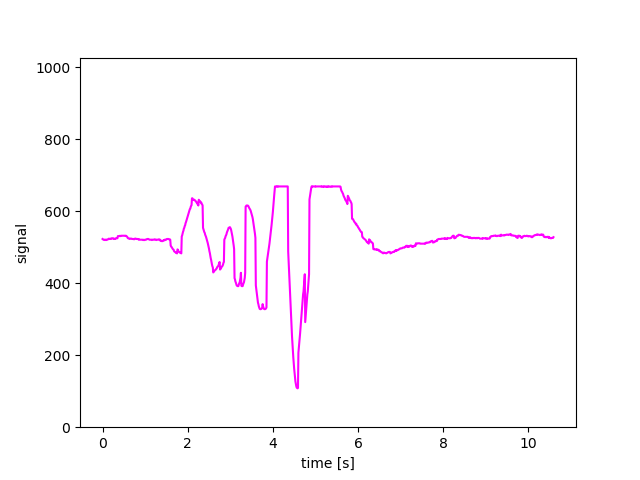
\includegraphics[width=0.3\textwidth]{../data/c4m_LR_3/c4m_LR_3_2.png}
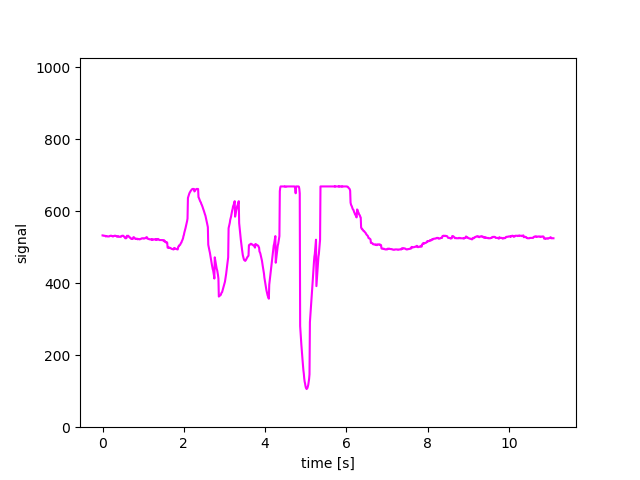
\includegraphics[width=0.3\textwidth]{../data/c4m_LR_3/c4m_LR_3_3.png}
\caption{c4m\_LR\_3.\label{fig:c4m_LR_3}}
\end{center}
\end{figure}

\begin{figure}[!ht]
\begin{center}
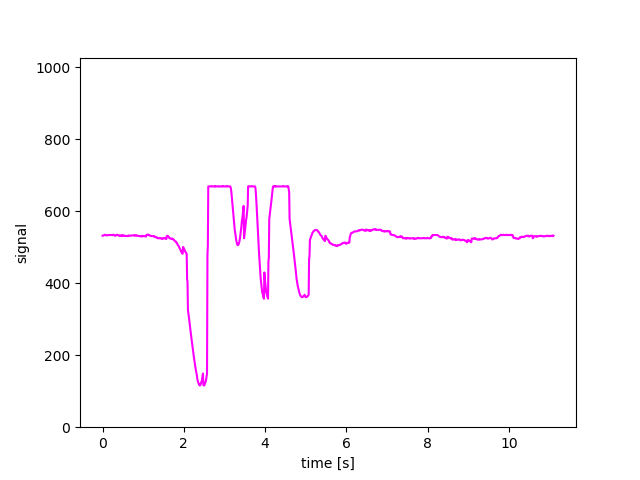
\includegraphics[width=0.3\textwidth]{../data/c4m_RL_1/c4m_RL_1_1.png}
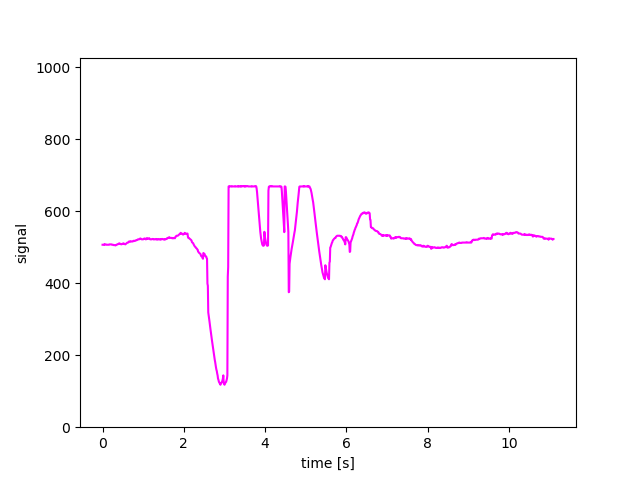
\includegraphics[width=0.3\textwidth]{../data/c4m_RL_1/c4m_RL_1_2.png}
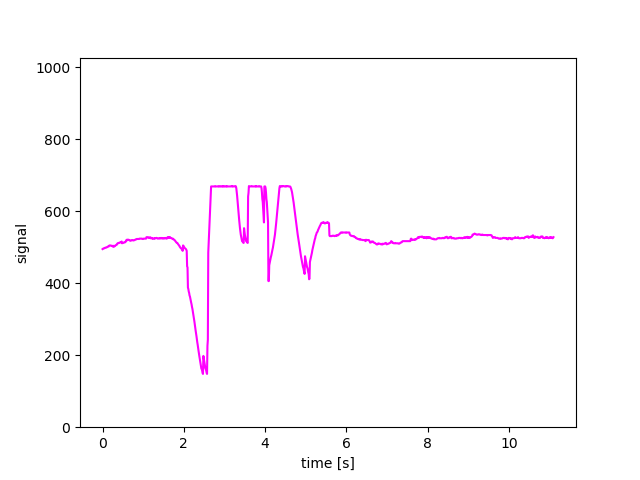
\includegraphics[width=0.3\textwidth]{../data/c4m_RL_1/c4m_RL_1_3.png}
\caption{c4m\_RL\_1.\label{fig:c4m_RL_1}}
\end{center}
\end{figure}

\begin{figure}[!ht]
\begin{center}
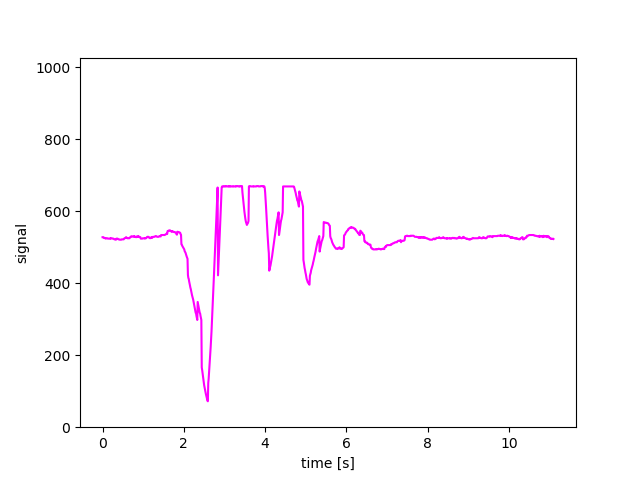
\includegraphics[width=0.3\textwidth]{../data/c4m_RL_2/c4m_RL_2_1.png}
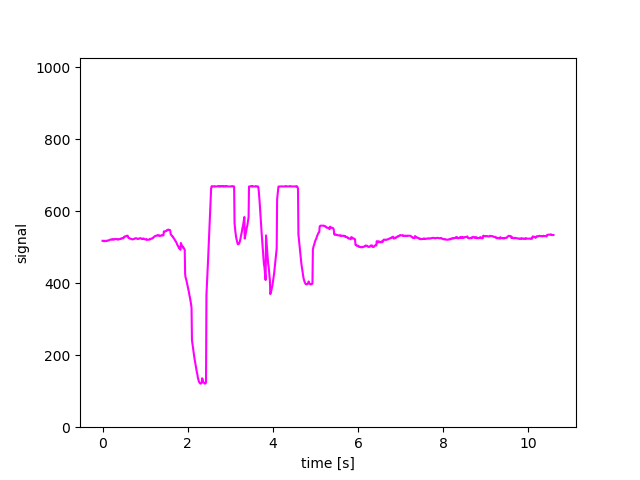
\includegraphics[width=0.3\textwidth]{../data/c4m_RL_2/c4m_RL_2_2.png}
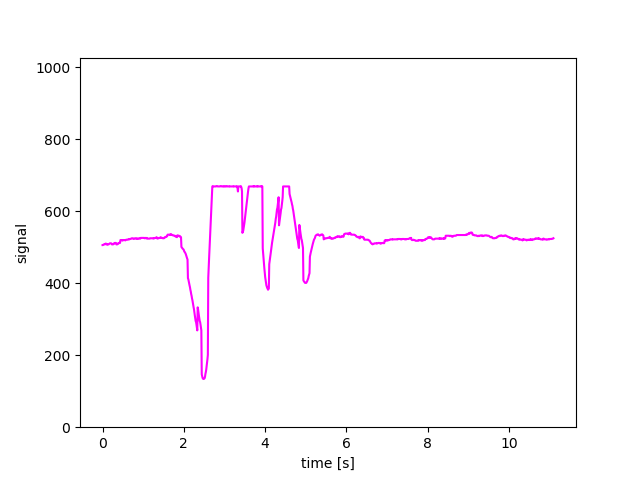
\includegraphics[width=0.3\textwidth]{../data/c4m_RL_2/c4m_RL_2_3.png}
\caption{c4m\_RL\_2.\label{fig:c4m_RL_2}}
\end{center}
\end{figure}

\begin{figure}[!ht]
\begin{center}
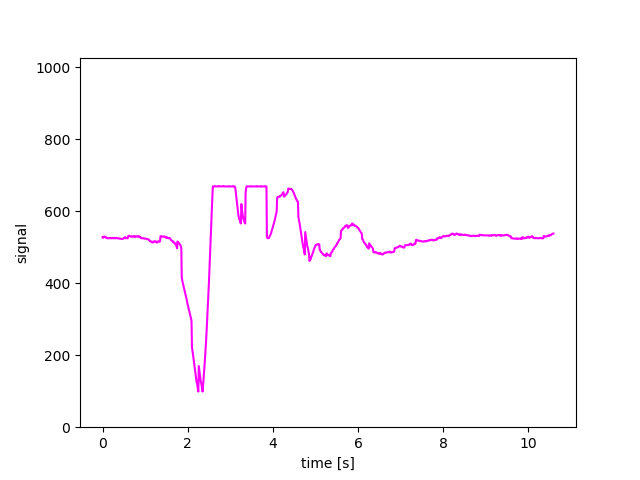
\includegraphics[width=0.3\textwidth]{../data/c4m_RL_3/c4m_RL_3_1.png}
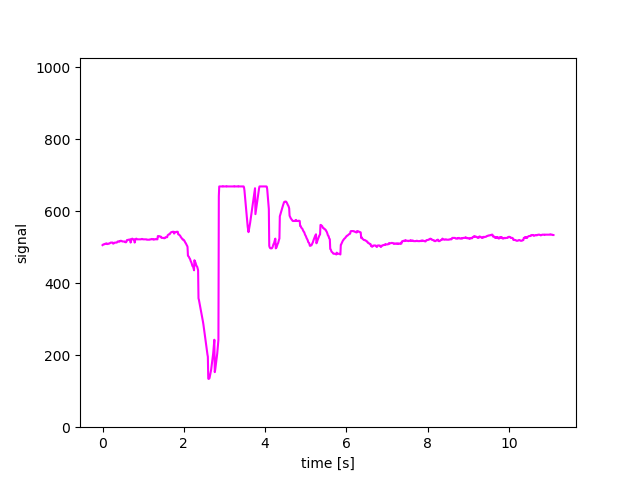
\includegraphics[width=0.3\textwidth]{../data/c4m_RL_3/c4m_RL_3_2.png}
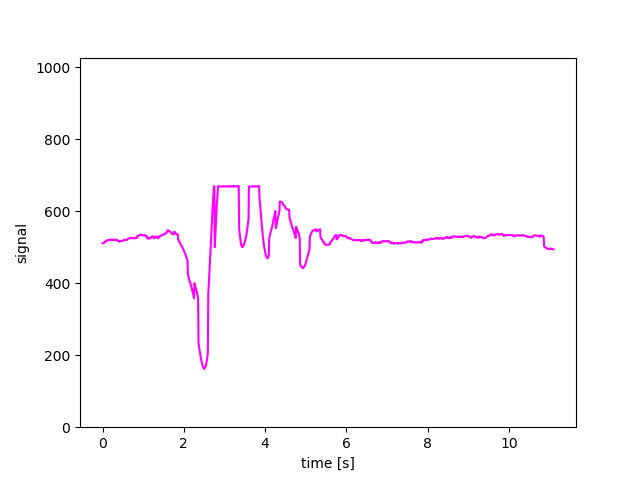
\includegraphics[width=0.3\textwidth]{../data/c4m_RL_3/c4m_RL_3_3.png}
\caption{c4m\_RL\_3.\label{fig:c4m_RL_3}}
\end{center}
\end{figure}

\begin{figure}[!ht]
\begin{center}
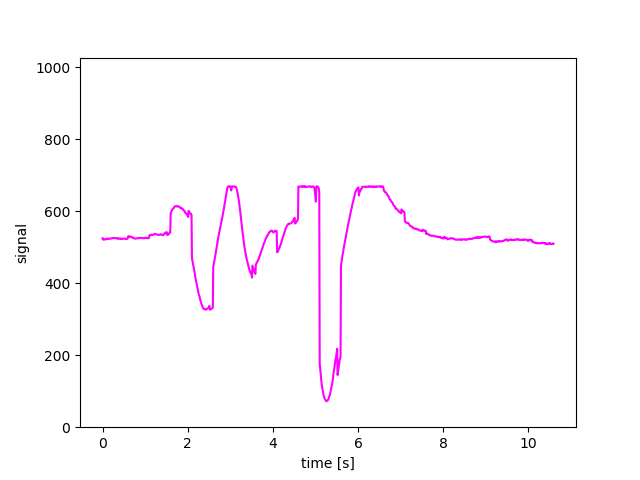
\includegraphics[width=0.3\textwidth]{../data/c5m_LR_1/c5m_LR_1_1.png}
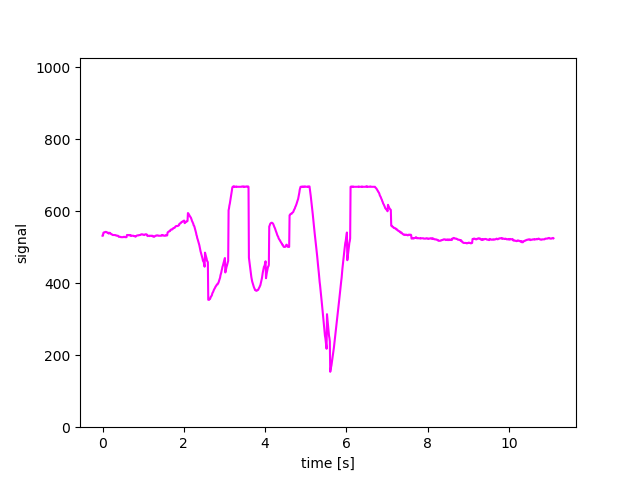
\includegraphics[width=0.3\textwidth]{../data/c5m_LR_1/c5m_LR_1_2.png}
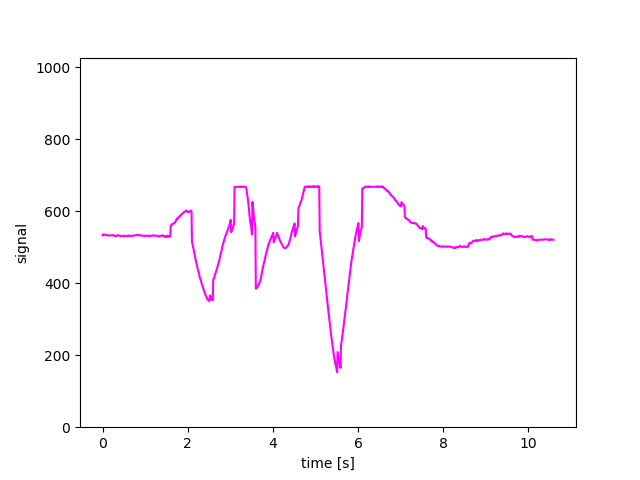
\includegraphics[width=0.3\textwidth]{../data/c5m_LR_1/c5m_LR_1_3.png}
\caption{c5m\_LR\_1.\label{fig:c5m_LR_1}}
\end{center}
\end{figure}

\begin{figure}[!ht]
\begin{center}
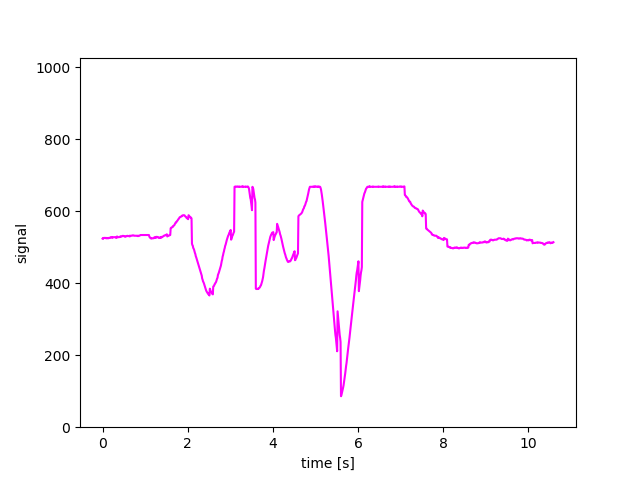
\includegraphics[width=0.3\textwidth]{../data/c5m_LR_2/c5m_LR_2_1.png}
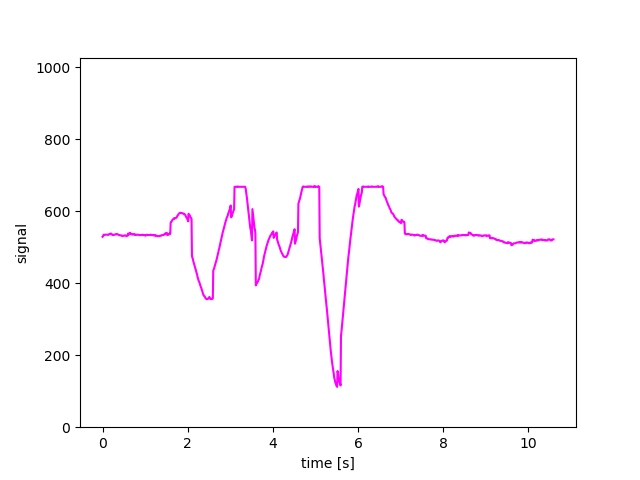
\includegraphics[width=0.3\textwidth]{../data/c5m_LR_2/c5m_LR_2_2.png}
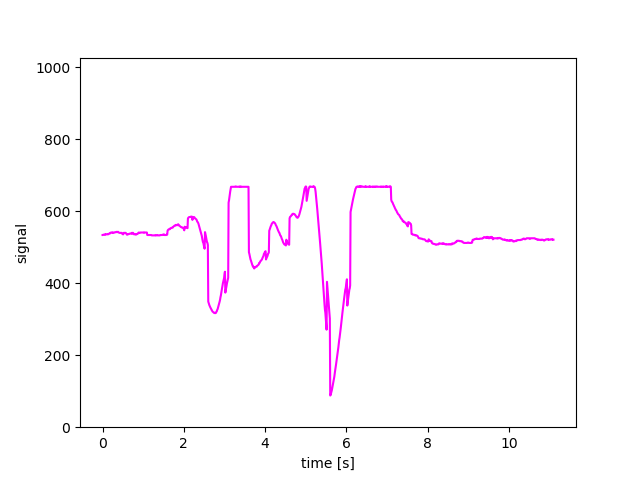
\includegraphics[width=0.3\textwidth]{../data/c5m_LR_2/c5m_LR_2_3.png}
\caption{c5m\_LR\_2.\label{fig:c5m_LR_2}}
\end{center}
\end{figure}

\begin{figure}[!ht]
\begin{center}
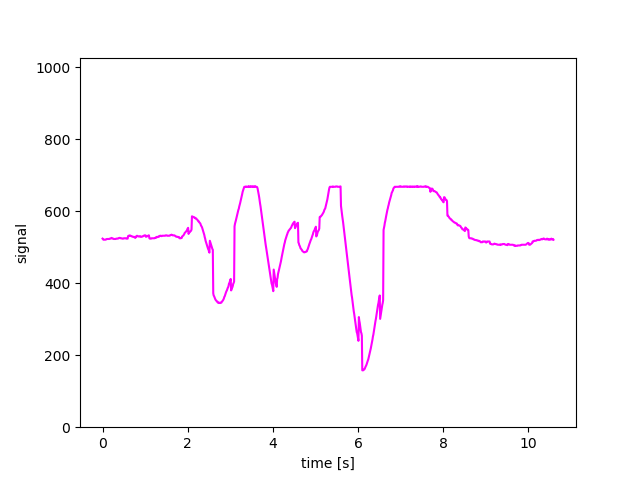
\includegraphics[width=0.3\textwidth]{../data/c5m_LR_3/c5m_LR_3_1.png}
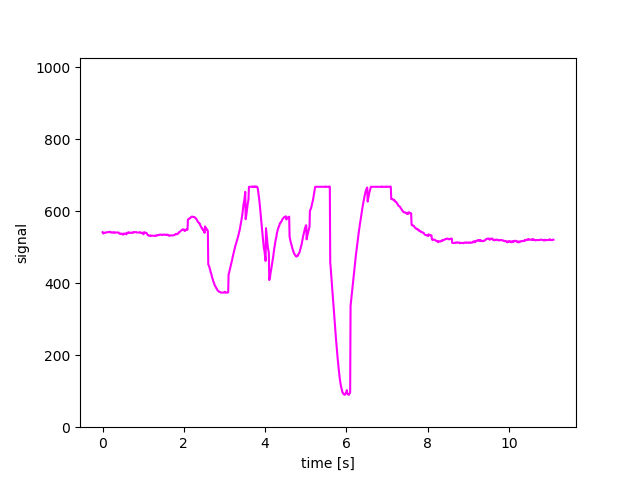
\includegraphics[width=0.3\textwidth]{../data/c5m_LR_3/c5m_LR_3_2.png}
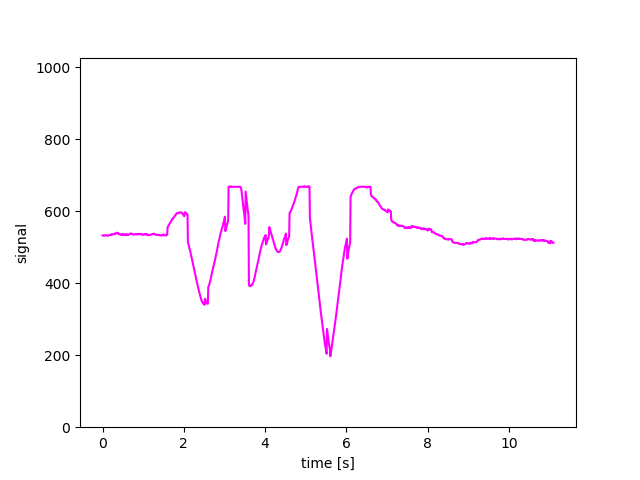
\includegraphics[width=0.3\textwidth]{../data/c5m_LR_3/c5m_LR_3_3.png}
\caption{c5m\_LR\_3.\label{fig:c5m_LR_3}}
\end{center}
\end{figure}

\begin{figure}[!ht]
\begin{center}
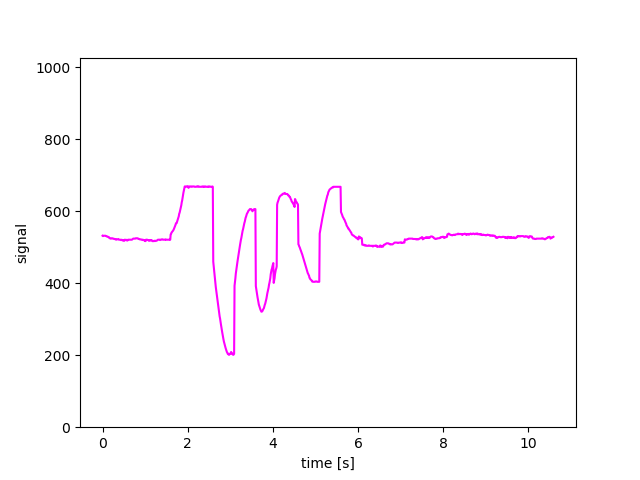
\includegraphics[width=0.3\textwidth]{../data/c5m_RL_1/c5m_RL_1_1.png}
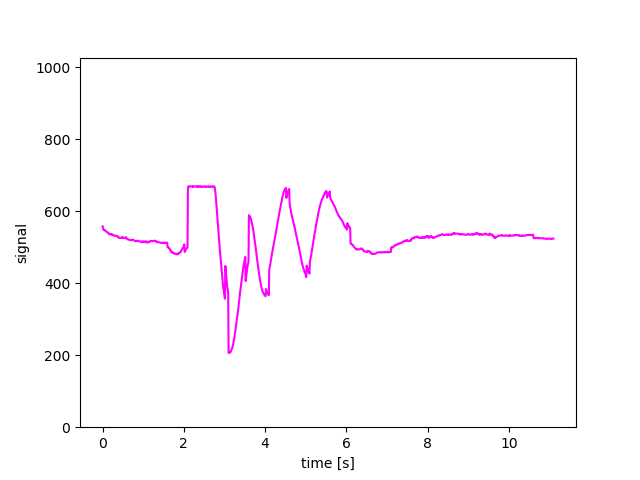
\includegraphics[width=0.3\textwidth]{../data/c5m_RL_1/c5m_RL_1_2.png}
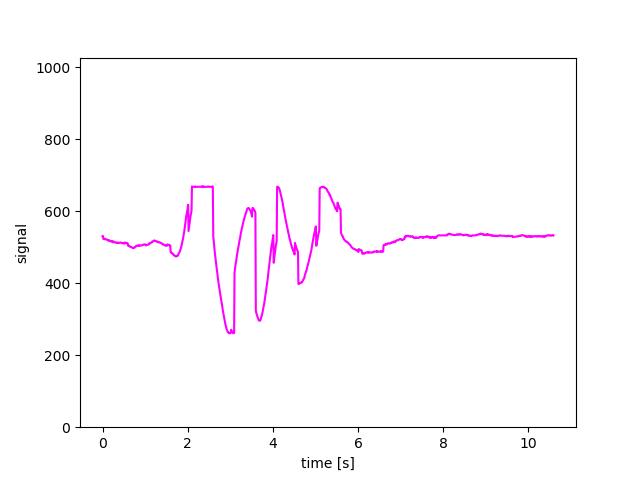
\includegraphics[width=0.3\textwidth]{../data/c5m_RL_1/c5m_RL_1_3.png}
\caption{c5m\_RL\_1.\label{fig:c5m_RL_1}}
\end{center}
\end{figure}

\begin{figure}[!ht]
\begin{center}
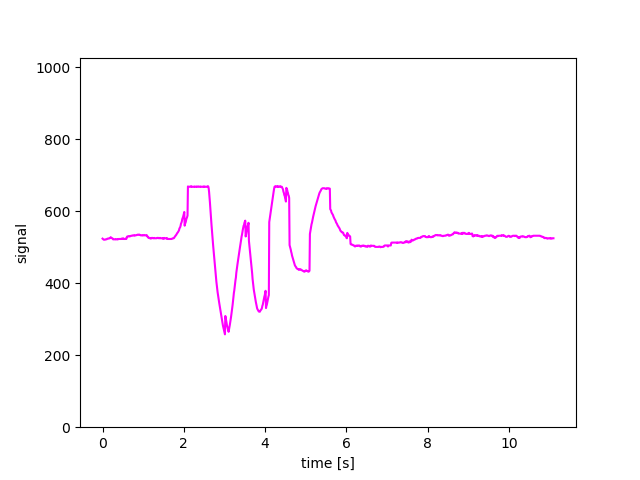
\includegraphics[width=0.3\textwidth]{../data/c5m_RL_2/c5m_RL_2_1.png}
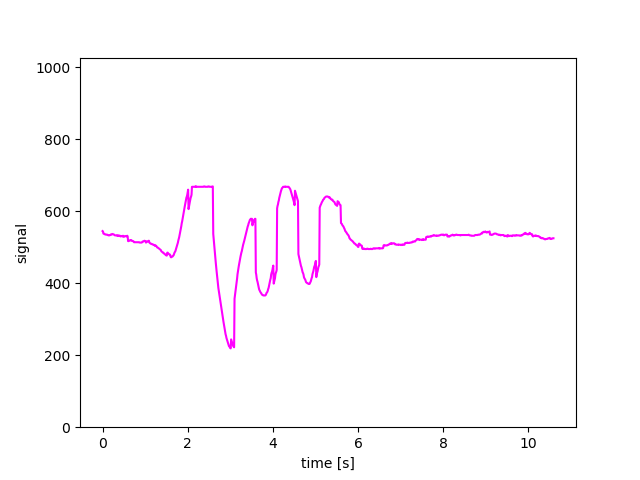
\includegraphics[width=0.3\textwidth]{../data/c5m_RL_2/c5m_RL_2_2.png}
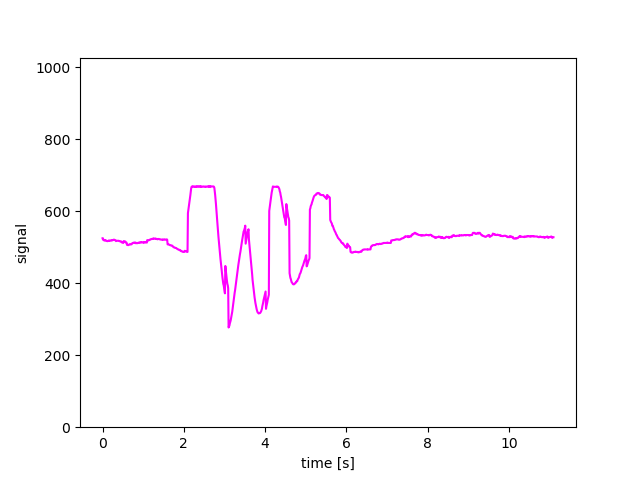
\includegraphics[width=0.3\textwidth]{../data/c5m_RL_2/c5m_RL_2_3.png}
\caption{c5m\_RL\_2.\label{fig:c5m_RL_2}}
\end{center}
\end{figure}

\begin{figure}[!ht]
\begin{center}
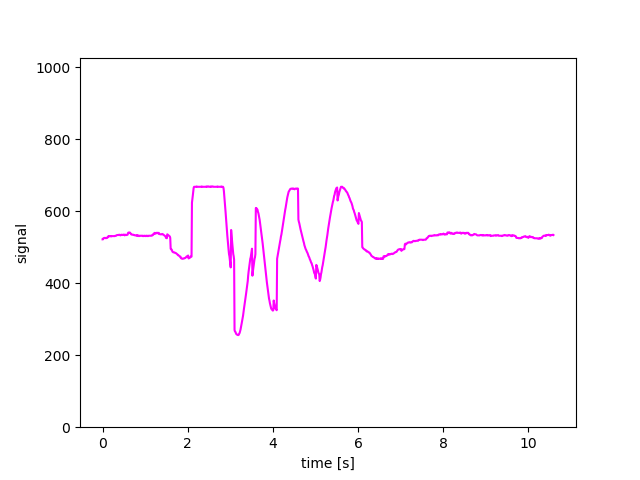
\includegraphics[width=0.3\textwidth]{../data/c5m_RL_3/c5m_RL_3_1.png}
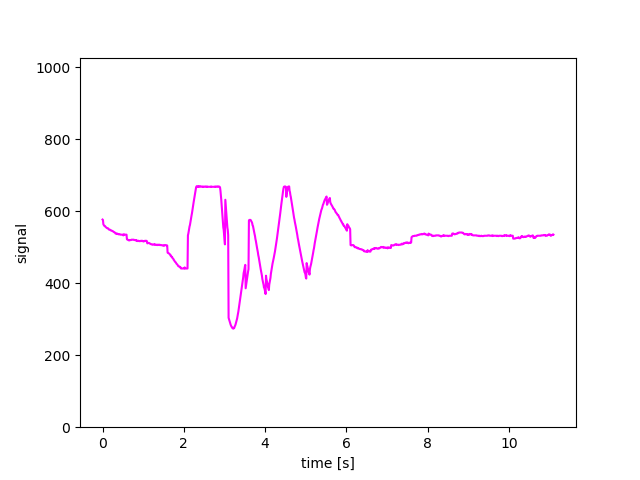
\includegraphics[width=0.3\textwidth]{../data/c5m_RL_3/c5m_RL_3_2.png}
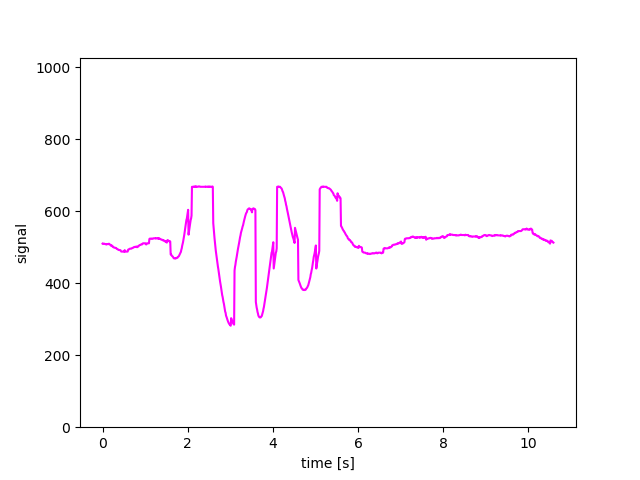
\includegraphics[width=0.3\textwidth]{../data/c5m_RL_3/c5m_RL_3_3.png}
\caption{c5m\_RL\_3.\label{fig:c5m_RL_3}}
\end{center}
\end{figure}

\begin{figure}[!ht]
\begin{center}
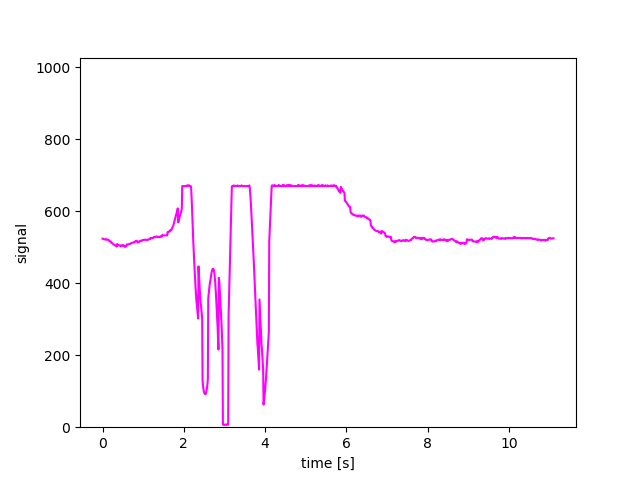
\includegraphics[width=0.3\textwidth]{../data/dFB_LR_1/dFB_LR_1_1.png}
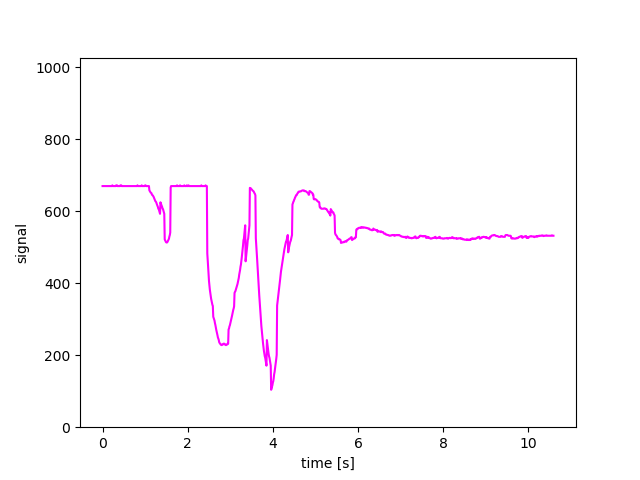
\includegraphics[width=0.3\textwidth]{../data/dFB_LR_1/dFB_LR_1_2.png}
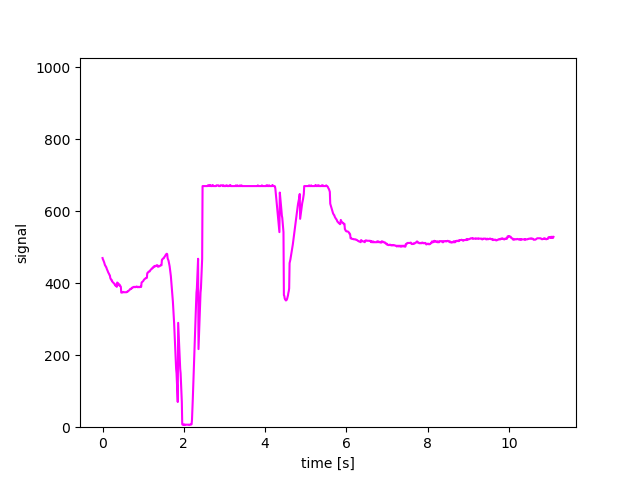
\includegraphics[width=0.3\textwidth]{../data/dFB_LR_1/dFB_LR_1_3.png}
\caption{dFB\_LR\_1.\label{fig:dFB_LR_1}}
\end{center}
\end{figure}

\begin{figure}[!ht]
\begin{center}
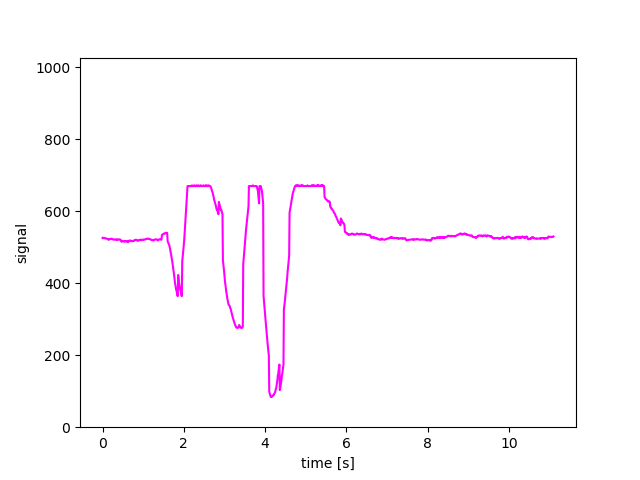
\includegraphics[width=0.3\textwidth]{../data/dFB_LR_2/dFB_LR_2_1.png}
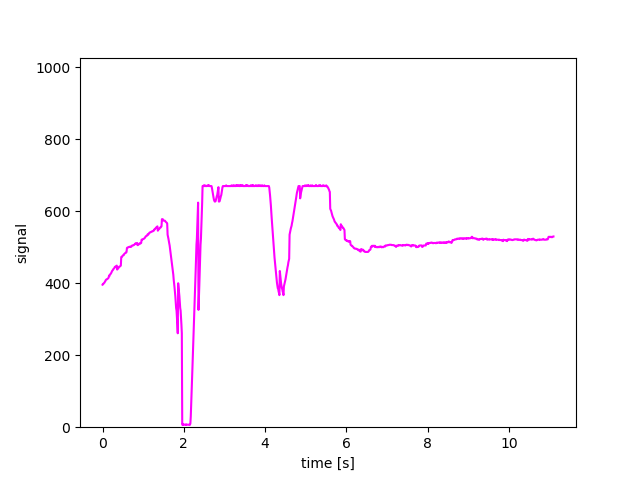
\includegraphics[width=0.3\textwidth]{../data/dFB_LR_2/dFB_LR_2_2.png}
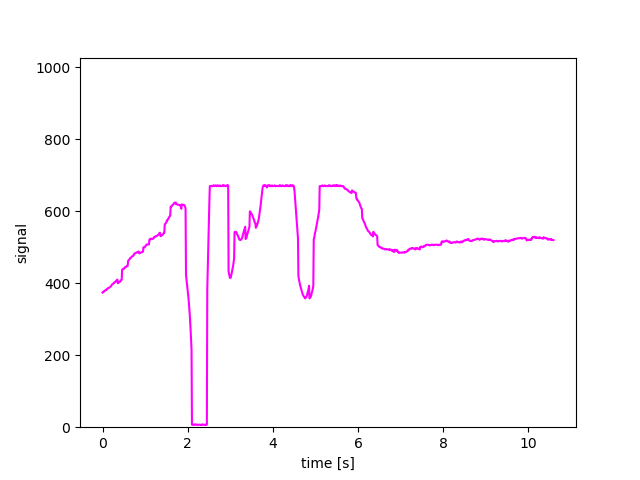
\includegraphics[width=0.3\textwidth]{../data/dFB_LR_2/dFB_LR_2_3.png}
\caption{dFB\_LR\_2.\label{fig:dFB_LR_2}}
\end{center}
\end{figure}

\begin{figure}[!ht]
\begin{center}
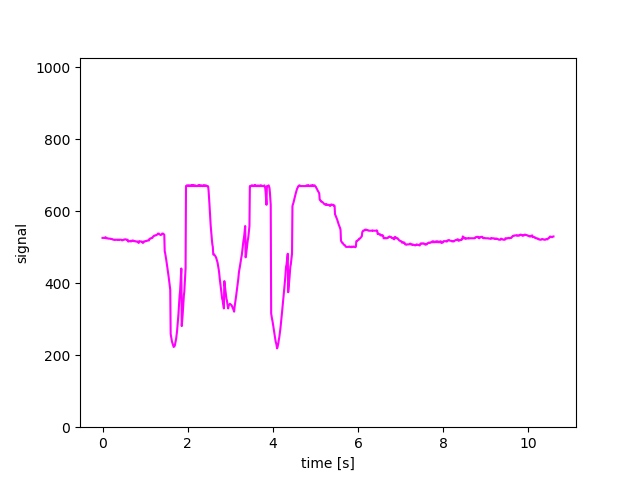
\includegraphics[width=0.3\textwidth]{../data/dFB_LR_3/dFB_LR_3_1.png}
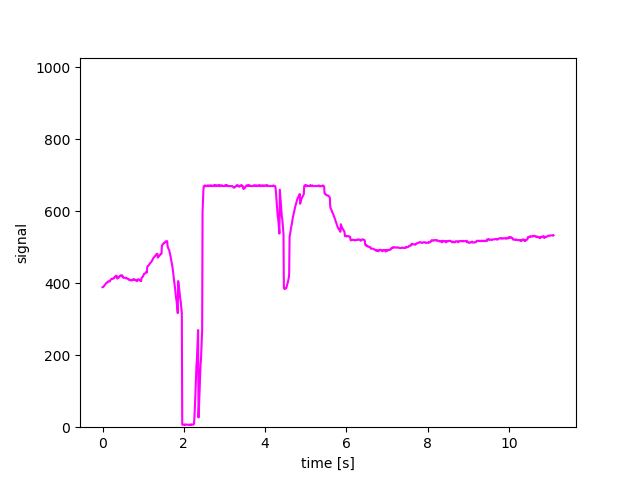
\includegraphics[width=0.3\textwidth]{../data/dFB_LR_3/dFB_LR_3_2.png}
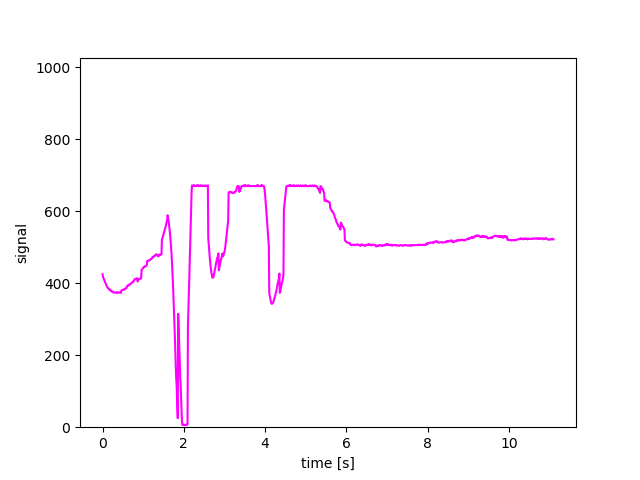
\includegraphics[width=0.3\textwidth]{../data/dFB_LR_3/dFB_LR_3_3.png}
\caption{dFB\_LR\_3.\label{fig:dFB_LR_3}}
\end{center}
\end{figure}

\begin{figure}[!ht]
\begin{center}
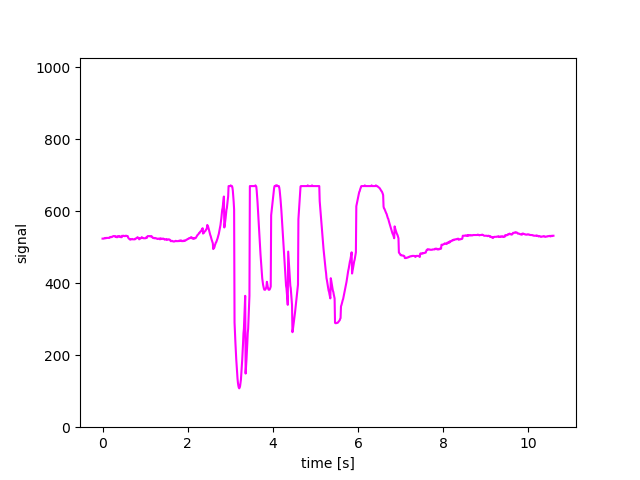
\includegraphics[width=0.3\textwidth]{../data/dFB_RL_1/dFB_RL_1_1.png}
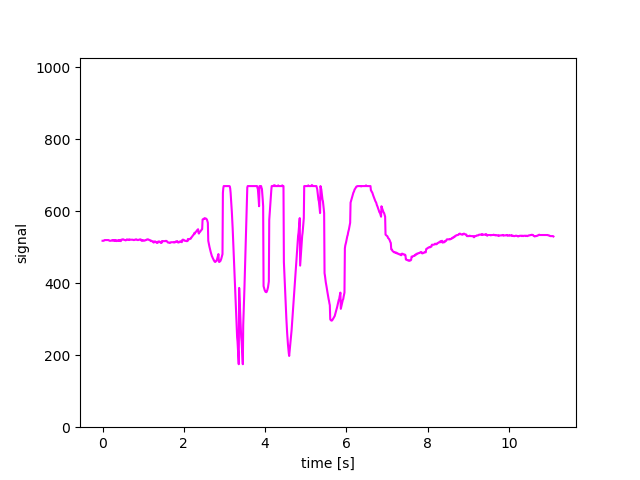
\includegraphics[width=0.3\textwidth]{../data/dFB_RL_1/dFB_RL_1_2.png}
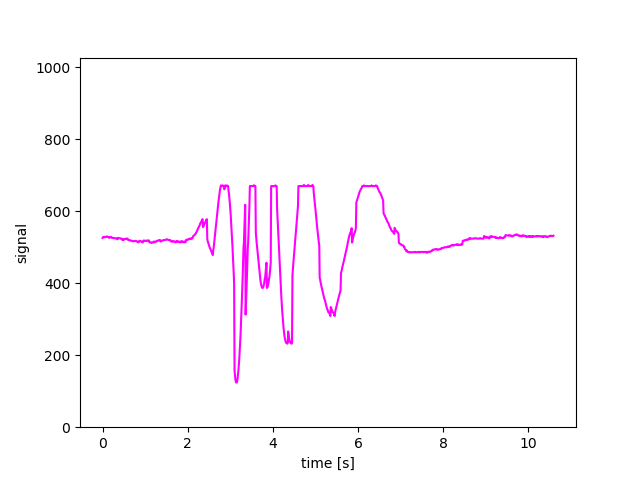
\includegraphics[width=0.3\textwidth]{../data/dFB_RL_1/dFB_RL_1_3.png}
\caption{dFB\_RL\_1.\label{fig:dFB_RL_1}}
\end{center}
\end{figure}

\begin{figure}[!ht]
\begin{center}
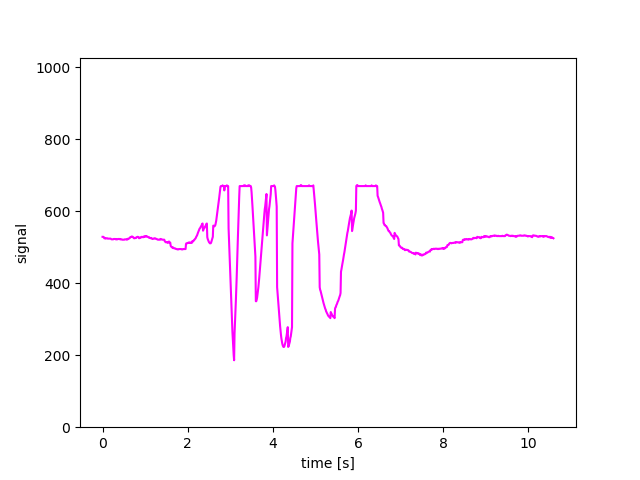
\includegraphics[width=0.3\textwidth]{../data/dFB_RL_2/dFB_RL_2_1.png}
\includegraphics[width=0.3\textwidth]{../data/dFB_RL_2/dFB_RL_2_2.png}
\includegraphics[width=0.3\textwidth]{../data/dFB_RL_2/dFB_RL_2_3.png}
\caption{dFB\_RL\_2.\label{fig:dFB_RL_2}}
\end{center}
\end{figure}

\begin{figure}[!ht]
\begin{center}
\includegraphics[width=0.3\textwidth]{../data/dFB_RL_3/dFB_RL_3_1.png}
\includegraphics[width=0.3\textwidth]{../data/dFB_RL_3/dFB_RL_3_2.png}
\includegraphics[width=0.3\textwidth]{../data/dFB_RL_3/dFB_RL_3_3.png}
\caption{dFB\_RL\_3.\label{fig:dFB_RL_3}}
\end{center}
\end{figure}


\begin{figure}[!ht]
\begin{center}
\includegraphics[width=0.3\textwidth]{../data/dBF_LR_1/dBF_LR_1_1.png}
\includegraphics[width=0.3\textwidth]{../data/dBF_LR_1/dBF_LR_1_2.png}
\includegraphics[width=0.3\textwidth]{../data/dBF_LR_1/dBF_LR_1_3.png}
\caption{dBF\_LR\_1.\label{fig:dBF_LR_1}}
\end{center}
\end{figure}

\begin{figure}[!ht]
\begin{center}
\includegraphics[width=0.3\textwidth]{../data/dBF_LR_2/dBF_LR_2_1.png}
\includegraphics[width=0.3\textwidth]{../data/dBF_LR_2/dBF_LR_2_2.png}
\includegraphics[width=0.3\textwidth]{../data/dBF_LR_2/dBF_LR_2_3.png}
\caption{dBF\_LR\_2.\label{fig:dBF_LR_2}}
\end{center}
\end{figure}

\begin{figure}[!ht]
\begin{center}
\includegraphics[width=0.3\textwidth]{../data/dBF_LR_3/dBF_LR_3_1.png}
\includegraphics[width=0.3\textwidth]{../data/dBF_LR_3/dBF_LR_3_2.png}
\includegraphics[width=0.3\textwidth]{../data/dBF_LR_3/dBF_LR_3_3.png}
\caption{dBF\_LR\_3.\label{fig:dBF_LR_3}}
\end{center}
\end{figure}

\begin{figure}[!ht]
\begin{center}
\includegraphics[width=0.3\textwidth]{../data/dBF_RL_1/dBF_RL_1_1.png}
\includegraphics[width=0.3\textwidth]{../data/dBF_RL_1/dBF_RL_1_2.png}
\includegraphics[width=0.3\textwidth]{../data/dBF_RL_1/dBF_RL_1_3.png}
\caption{dBF\_RL\_1.\label{fig:dBF_RL_1}}
\end{center}
\end{figure}

\begin{figure}[!ht]
\begin{center}
\includegraphics[width=0.3\textwidth]{../data/dBF_RL_2/dBF_RL_2_1.png}
\includegraphics[width=0.3\textwidth]{../data/dBF_RL_2/dBF_RL_2_2.png}
\includegraphics[width=0.3\textwidth]{../data/dBF_RL_2/dBF_RL_2_3.png}
\caption{dBF\_RL\_2.\label{fig:dBF_RL_2}}
\end{center}
\end{figure}

\begin{figure}[!ht]
\begin{center}
\includegraphics[width=0.3\textwidth]{../data/dBF_RL_3/dBF_RL_3_1.png}
\includegraphics[width=0.3\textwidth]{../data/dBF_RL_3/dBF_RL_3_2.png}
\includegraphics[width=0.3\textwidth]{../data/dBF_RL_3/dBF_RL_3_3.png}
\caption{dBF\_RL\_3.\label{fig:dBF_RL_3}}
\end{center}
\end{figure}

\begin{figure}[!ht]
\begin{center}
\includegraphics[width=0.3\textwidth]{../data/e_1/e_1_1.png}
\includegraphics[width=0.3\textwidth]{../data/e_1/e_1_2.png}
\includegraphics[width=0.3\textwidth]{../data/e_1/e_1_3.png}
\caption{e\_1.\label{fig:e_1}}
\end{center}
\end{figure}

\begin{figure}[!ht]
\begin{center}
\includegraphics[width=0.3\textwidth]{../data/e_2/e_2_1.png}
\includegraphics[width=0.3\textwidth]{../data/e_2/e_2_2.png}
\includegraphics[width=0.3\textwidth]{../data/e_2/e_2_3.png}
\caption{e\_2.\label{fig:e_2}}
\end{center}
\end{figure}

\begin{figure}[!ht]
\begin{center}
\includegraphics[width=0.3\textwidth]{../data/e_3/e_3_1.png}
\includegraphics[width=0.3\textwidth]{../data/e_3/e_3_2.png}
\includegraphics[width=0.3\textwidth]{../data/e_3/e_3_3.png}
\caption{e\_3.\label{fig:e_3}}
\end{center}
\end{figure}

\begin{figure}[!ht]
\begin{center}
\includegraphics[width=0.3\textwidth]{../data/e_4/e_4_1.png}
\includegraphics[width=0.3\textwidth]{../data/e_4/e_4_2.png}
\includegraphics[width=0.3\textwidth]{../data/e_4/e_4_3.png}
\caption{e\_4.\label{fig:e_4}}
\end{center}
\end{figure}

\begin{figure}[!ht]
\begin{center}
\includegraphics[width=0.3\textwidth]{../data/e_5/e_5_1.png}
\includegraphics[width=0.3\textwidth]{../data/e_5/e_5_2.png}
\includegraphics[width=0.3\textwidth]{../data/e_5/e_5_3.png}
\caption{e\_5.\label{fig:e_5}}
\end{center}
\end{figure}

\begin{figure}[!ht]
\begin{center}
\includegraphics[width=0.3\textwidth]{../data/e_6/e_6_1.png}
\includegraphics[width=0.3\textwidth]{../data/e_6/e_6_2.png}
\includegraphics[width=0.3\textwidth]{../data/e_6/e_6_3.png}
\caption{e\_6.\label{fig:e_6}}
\end{center}
\end{figure}

\begin{figure}[!ht]
\begin{center}
\includegraphics[width=0.3\textwidth]{../data/e_7/e_7_1.png}
\includegraphics[width=0.3\textwidth]{../data/e_7/e_7_2.png}
\includegraphics[width=0.3\textwidth]{../data/e_7/e_7_3.png}
\caption{e\_7.\label{fig:e_7}}
\end{center}
\end{figure}

\begin{figure}[!ht]
\begin{center}
\includegraphics[width=0.3\textwidth]{../data/e_8/e_8_1.png}
\includegraphics[width=0.3\textwidth]{../data/e_8/e_8_2.png}
\includegraphics[width=0.3\textwidth]{../data/e_8/e_8_3.png}
\caption{e\_8.\label{fig:e_8}}
\end{center}
\end{figure}

%\begin{subequations}
%\begin{equation}
%    \alpha_A = \frac{2b_A}{r} = \frac{5}{11} = \underline{0.4545}
%\end{equation}
%\begin{equation}
%    \alpha_B = \frac{2b_A + 2b_B}{r} = \frac{5 + 10}{11} = \underline{1.3636}
%\end{equation}
%\begin{equation}
%    \alpha_C = \frac{2b_A + 2b_B + 2b_C}{r} = \frac{5 + 10 + 8}{11} = \underline{2.0909}
%\end{equation}
%\end{subequations}
%\begin{subequations}
%\begin{equation}
%    \varphi_1 = \frac{\alpha_C - \alpha_B}{2} = \frac{2.0909 - 1.3636}{2} = 0.36365
%\end{equation}
%\begin{equation}
%    \varphi_2 = \frac{\alpha_B - \alpha_A}{2} = \frac{1.3636 - 0.4545}{2} = 0.45455
%\end{equation}
%\begin{equation}
%    \varphi_3 = \frac{\alpha_A}{2} = \frac{0.4545}{2} = 0.22725
%\end{equation}
%\end{subequations}

%During the movement around the sensor with circular trajectory of radius $r_X$,
%the sectors are being crossed in the order $\varphi_1$, $\varphi_2$, $\varphi_3$,
%$\varphi_3^{'}$, $\varphi_2^{'}$, $\varphi_1^{'}$. The length of a sector $l$ is

%\begin{equation}
%  l = \varphi r
%\end{equation}

%The measurement was done in a room with width $w = 7.63~m$, $w_R = 4.25~m$ on the right
%and $w_L = 3.38~m$ from the left. The radiuses of circular trajectories were $3~m$, $6~m$, $9~m$ and $12~m$.

%To calculate maximal possible angle equation at figure \ref{fig:maxangle} can be used, $w$ is a distance of
%the sensor and a side wall, $r$ is a distance of the object we want to calculate the maximal angle of.

%\begin{figure}[ht!]
%\begin{equation}
%\varphi_{max}(w, r) = \text{min}(\frac{\alpha_C}{2}, 
%  \begin{cases}
%    \text{arcsin}(\frac{w}{r}) & \frac{w}{r} \in (0 ; 1) \\ 
%    \infty                      & \text{otherwise}
%  \end{cases}
%)
%\end{equation}
%\caption{Instantaneous maximal angle. \label{fig:maxangle}}
%\end{figure}

%\begin{subequations}
%\begin{equation}
%\varphi_{max}(3.38~m, 3~m) = \text{min}(\frac{2.0909}{2}, \infty) =  1.04545
%\end{equation}
%\begin{equation}
%\varphi_{max}(4.25~m, 3~m) = \text{min}(1.04545, \infty) =  1.04545
%\end{equation}
%\end{subequations}

%\begin{subequations}
%\begin{equation}
%\varphi_{max}(3.38~m, 6~m) = \text{min}(1.04545, \text{arcsin}(\frac{3.38}{6})) = 0.59841
%\end{equation}
%\begin{equation}
%\varphi_{max}(4.25~m, 6~m) = \text{min}(1.04545, \text{arcsin}(\frac{4.25}{6})) = 0.78713
%\end{equation}
%\end{subequations}

%\begin{subequations}
%\begin{equation}
%\varphi_{max}(3.38~m, 9~m) = \text{min}(1.04545, \text{arcsin}(\frac{3.38}{9})) = 0.385
%\end{equation}
%\begin{equation}
%\varphi_{max}(4.25~m, 9~m) = \text{min}(1.04545, \text{arcsin}(\frac{4.25}{9})) = 0.49181
%\end{equation}
%\end{subequations}



%\begin{subequations}
%\begin{equation}
%\varphi_{max}(3.38~m, 12~m) = \text{min}(1.04545, \text{arcsin}(\frac{3.38}{12})) = 0.28553
%\end{equation}
%\begin{equation}
%\varphi_{max}(4.25~m, 12~m) = \text{min}(1.04545, \text{arcsin}(\frac{4.25}{12})) = 0.36202
%\end{equation}
%\end{subequations}

%This means, that walking around the circle should generate signal that will be scaled with
%the distance of the object from the sensor.

\chapter{CD Structure}
Structure of files in the attached CD is following:
\begin{itemize}
\item \texttt{monitor/} Classification server source codes.
\item \texttt{monitor/env/} Run environment.
\item \texttt{monitor/classifiers/} Trained classifier and service scripts.
\item \texttt{module/} Module program and device design.
\item \texttt{data/} Training data.
\item \texttt{xbenes49.pdf} Text of thesis.
\item \texttt{README.md} Description.
\item \texttt{pirstd.pdf} Documentation of PIR STD.
\end{itemize}





